\documentclass[11pt]{article}
\usepackage[T1]{fontenc}
\usepackage[utf8]{inputenc}
\usepackage{lmodern,microtype,amsmath,amssymb,amsthm,mathtools}
\usepackage[a4paper,margin=28mm]{geometry}
\usepackage{xcolor,xurl,enumitem,booktabs,tikz}
\usetikzlibrary{arrows.meta}
\usepackage[unicode,colorlinks=true,linkcolor=blue!45!black,citecolor=green!35!black,urlcolor=blue!55!black]{hyperref}
\setlength{\emergencystretch}{2em}
\numberwithin{equation}{section}
\newtheorem{theorem}{Theorem}[section]
\newtheorem{proposition}[theorem]{Proposition}
\newtheorem{lemma}[theorem]{Lemma}
\newtheorem{corollary}[theorem]{Corollary}
\theoremstyle{definition}\newtheorem{definition}[theorem]{Definition}
\theoremstyle{remark}\newtheorem{remark}[theorem]{Remark}
\newcommand{\ii}{\mathrm i}
\newcommand{\Rea}{\operatorname{Re}}
\newcommand{\Ima}{\operatorname{Im}}
\title{Oscillatory filling sums with independently long twists}
\author{}
\date{}
\begin{document}
\maketitle
\begin{abstract}
An exact finite Hermite functional can be written as a sum of oscillatory
integrals indexed by nonzero integer Fourier charges. We prove an
asymptotic formula for the whole sum from two source estimates: a
nonvanishing holomorphic expansion near the complete point and a strict
spectral gap away from it. The twist numbers are independently signed,
sufficiently large integers, fixed before the level tends to infinity.
The proof first bounds all distant charges on the original intervals,
including the paired endpoint contributions. Only the remaining finite
set is localized near its stationary points. The charges of magnitude
one contribute equally, while every other charge is exponentially smaller.
The resulting amplitude is nonzero and retains the finite-level action.
We state the application to marked knot sources with its local analytic
and geometric inputs explicit; this paper does not prove those inputs or
estimate the other degree regions of the invariant.
\end{abstract}

\section{The question and the hypotheses}

The volume conjecture concerns an oscillatory invariant, so an estimate
for a positive sum of absolute values does not determine its limit. Even
after a promising geometric contribution has been isolated, one must
show that it occurs on the original contour and survives the other terms
of the same sum. We address one precise part of that problem: the passage
from a local holomorphic source expansion to its entire Fourier filling
sum.

The motivating finite functional is defined in
\cite{FinitePaper}. It includes first derivatives at double spectral
roots, as well as the value at an odd simple root. Its Fourier
representation involves every nonzero integer charge. Absolute
convergence for each fixed level is insufficient for an asymptotic
argument: the constants in such a convergence estimate can grow
exponentially with the level. We therefore prove a separate estimate
for the infinite set of distant charges before restricting any integral
to a small neighborhood.

Our contour and Gaussian arguments are instances of the classical
saddle-point method; see, for example, \cite[\S2.4]{DLMF} and
\cite{Hormander}. The proof below gives the contour, its side faces,
the determinant branch and the charge estimates explicitly. These
details are needed to distinguish the complete filling sum from an
arbitrarily chosen local integral.

Fix an integer $r\ge1$. For every integer $N\ge3$, let
$P_N(\sigma_1,\ldots,\sigma_r)$ be a complex polynomial of degree at
most $N-1$ in each separate variable. Put
\begin{equation}\label{of:source}
 C_N(\delta)=P_N(-2\cos(2\pi\delta_1),\ldots,
                         -2\cos(2\pi\delta_r)),\qquad
 \delta=(\delta_1,\ldots,\delta_r)\in\mathbb C^r.
\end{equation}
Thus $C_N$ is entire, one-periodic and even in each variable separately.
No bound on its total degree smaller than $r(N-1)$ is assumed.
Write $I=[-1/2,1/2]$, and use Euclidean norm for real vectors and
maximum norm when specifying polydisks.

We make the following two analytic assumptions. Their constants do not
depend on the later twist numbers.

\begin{enumerate}[label=(\roman*)]
\item\label{of:Hlocal}
There is a fixed complex polydisk about zero, a real exponent $\alpha$,
unit scalars $\varepsilon_N$, and holomorphic functions $A_N,a_N,e_N$
on that polydisk such that
\begin{equation}\label{of:packet}
 C_N(\delta)=\varepsilon_N N^\alpha a_N(\delta)
                   e^{NA_N(\delta)}(1+e_N(\delta)),
 \qquad \sup|e_N|=O(N^{-1}).
\end{equation}
The functions $A_N$ are separately even and real on the real polydisk.
They converge locally uniformly to a holomorphic function $A_0$, and
$a_N$ converge locally uniformly to a holomorphic function $a$ with
$a(0)\ne0$. Finally, for real numbers $\Phi$ and $c_j>0$,
\begin{equation}\label{of:hessian}
 A_0(0)=\Phi,\qquad A_0''(0)=-2\operatorname{diag}(c_1,\ldots,c_r).
\end{equation}
All functions are considered on smaller closed polydisks when a
uniform bound is used. Cauchy's formula then gives convergence and
bounds for every fixed derivative. Shrinking the disk makes $a$ and,
for all large $N$, $a_N$ nonzero there.

\item\label{of:Hgap}
For each sufficiently small $\eta>0$ there are numbers
$\tau_\eta,\gamma_\eta>0$ such that, for all large $N$,
\begin{equation}\label{of:gap}
 |C_N(x+\ii y)|\le e^{N(\Phi-\gamma_\eta)}
 \quad\text{when }x\in I^r,\quad
 \max_j|x_j|\ge\eta,\quad \max_j|y_j|\le\tau_\eta.
\end{equation}
The bound is for the shared polynomial $P_N$ itself. Separate estimates
for its local factors are not a substitute for this hypothesis.
\end{enumerate}

The restriction to sufficiently small $\eta$ loses nothing in later
uses at an endpoint: an endpoint also lies outside any such small
neighborhood. Periodicity permits equivalent real representatives.
Bounds for fixed derivatives follow on smaller strips by Cauchy's
formula, keeping one separated real coordinate at distance at least
$\eta/2$ from the origin modulo the period.

For a fixed tuple $\boldsymbol n=(n_1,\ldots,n_r)$ of nonzero signed
integers, set $d=N-1$, $q=e^{\pi\ii/N}$ and
\begin{equation}\label{of:scalar}
 \Gamma_N(\boldsymbol n)
   =\exp\left(\frac{\pi\ii d^2}{4N}\sum_j n_j\right).
\end{equation}
It has modulus one; the exponential specifies its lift without a
choice of fractional power. Define
\begin{equation}\label{of:period}
\begin{split}
 \mathcal I_N(\boldsymbol n)
 ={}&\Gamma_N(\boldsymbol n)(-\ii)^r
 \sum_{\ell\in(\mathbb Z\setminus\{0\})^r}
       \left(\prod_j\ell_j\right)(-1)^{(N+1)\sum_j\ell_j}\\
 &\quad\times\int_{I^r}C_N(\delta)
       \prod_j\sin(2\pi\delta_j)
       \exp\left\{N\sum_j
          (\pi\ii n_j\delta_j^2+2\pi\ii\ell_j\delta_j)\right\}
                       d\delta.
\end{split}
\end{equation}
Section~\ref{of:fourier} proves absolute convergence at each fixed
$N$ and identifies this expression with the finite Hermite functional.
The term \emph{charge} will mean precisely an index $\ell_j$ in this sum.

\begin{theorem}[The whole filling sum]\label{of:main}
Under \eqref{of:source}--\eqref{of:gap}, there is $n_0$ such that the
following holds for every fixed signed integer tuple with
$|n_j|\ge n_0$ for all $j$. For all sufficiently large $N$, the phase
\begin{equation}\label{of:phase}
 F_{N,\ell}(\delta)=A_N(\delta)
            +\pi\ii\sum_j n_j\delta_j^2
            +2\pi\ii\sum_j\ell_j\delta_j
\end{equation}
has a unique critical point near zero for $\ell=\mathbf1=(1,\ldots,1)$.
Write that point as $z_N$, and put
\[
 S_N=F_{N,\mathbf1}(z_N),\qquad
 Q_N=-F_{N,\mathbf1}''(z_N).
\]
Then
\begin{equation}\label{of:asymptotic}
\begin{split}
 \mathcal I_N(\boldsymbol n)
 ={}&\Gamma_N\varepsilon_N(-1)^{(N+1)r}(-2\ii)^r
       (2\pi)^{r/2}N^{\alpha-r/2}\\
 &\quad\times\frac{a_N(z_N)\prod_j\sin(2\pi z_{N,j})}
                         {\sqrt{\det Q_N}}
       e^{NS_N}\left(1+O_{\boldsymbol n}(N^{-1})
                        +O_{\boldsymbol n}(e^{-\kappa_{\boldsymbol n}N})\right)
\end{split}
\end{equation}
for some $\kappa_{\boldsymbol n}>0$. The square root is the Gaussian
branch on symmetric matrices with positive definite real part.
The critical points, actions and normalized coefficients converge;
the coefficient in the second line, excluding $e^{NS_N}$, converges to
a nonzero number. In particular $\mathcal I_N$ is eventually nonzero and
\begin{equation}\label{of:rate}
 \lim_{N\to\infty}\frac1N\log|\mathcal I_N(\boldsymbol n)|
                         =\Rea S_0,
 \qquad S_0=\lim_{N\to\infty}S_N.
\end{equation}
Moreover $\Phi-\Rea S_0=O(\sum_j n_j^{-2})$ as the independent
magnitudes tend to infinity. Neither the threshold nor this last
bound imposes a restriction on their ratios.
\end{theorem}

The constants in the relative error may depend on the fixed tuple.
The theorem makes no assertion when the twists grow with $N$.
The finite $S_N$ remains inside the exponential. Convergence
$S_N\to S_0$ alone would not justify replacing $e^{NS_N}$ by
$e^{NS_0}$ in a relative asymptotic formula.

\subsection{An elementary example}

The two assumptions can already be checked for the polynomial sequence
\[
 P_N(\sigma)=\prod_{j=1}^r
                   (\beta_j-\gamma_j\sigma_j/2)^{N-1},
                  \qquad \beta_j>\gamma_j>0 .
\]
Here
\[
 C_N(\delta)=
   \prod_j(\beta_j+\gamma_j\cos(2\pi\delta_j))^{N-1}.
\]
Choose the logarithm that is real at zero. On a fixed sufficiently
small complex polydisk the factors are nonzero, and assumption
\ref{of:Hlocal} holds exactly with $\alpha=0$, $\varepsilon_N=1$,
$a_N=1$, $e_N=0$ and
\[
 A_N(\delta)=(1-N^{-1})
            \sum_j\log(\beta_j+\gamma_j\cos(2\pi\delta_j)).
\]
In particular,
\[
 \Phi=\sum_j\log(\beta_j+\gamma_j),\qquad
 c_j=\frac{2\pi^2\gamma_j}{\beta_j+\gamma_j}>0 .
\]
On the real torus each factor is positive and attains its maximum
only at $\delta_j=0$ modulo one. Compactness gives a number $g>0$
for which the product is at most $e^{\Phi-g}$ outside any fixed
neighborhood of zero. Continuity bounds its modulus by
$e^{\Phi-g/2}$ in a sufficiently thin complex strip. For all large
$N$, its $(N-1)$st power is at most $e^{N(\Phi-g/4)}$.
This proves assumption~\ref{of:Hgap}. The theorem therefore applies to the
entire filling sum of this explicit sequence. This example is not
asserted to be a knot invariant. It illustrates why the local
expansion and the global gap are distinct hypotheses and how each
can be verified.

\section{The exact Fourier representation}\label{of:fourier}

We explain the normalization before estimating the sum. For a polynomial
$H$ of degree at most $d$, the finite filling functional of
\cite[Section 3]{FinitePaper} has the midpoint formula
\begin{equation}\label{of:midpoint}
 \mathcal L_N^nH=-N^{-2}\sum_{k=0}^{N-1}g'(\phi_k),\qquad
 \phi_k=\frac{(2k+1)\pi}{N},
\end{equation}
where
\[
 g(\phi)=\sin\phi\,q^{nd^2/4}
         \exp\left(\frac{\ii nN(\phi-\pi)^2}{4\pi}\right)
         H(2\cos\phi),\qquad 0\le\phi\le2\pi.
\]
The functional in \eqref{of:midpoint} retains the derivative at each
double root; it is not evaluation only at the distinct roots.
Its finite proof is the only quantum-algebra input to this section.

At the endpoints, $g=0$ and $g'(0)=g'(2\pi)$. The equality follows
because the derivative of the sine is the only surviving term and
the remaining factors have the same endpoint values. Let
\[
 \widehat g_k=\frac1{2\pi}\int_0^{2\pi}g(\phi)e^{-\ii k\phi}\,d\phi.
\]
Three integrations by parts, retaining the boundary difference in
$g''$, give $\widehat g_k=O_{N,n}(|k|^{-3})$. Consequently the Fourier
series of $g'$ is absolutely convergent, with coefficients
$\ii k\widehat g_k$, and represents its continuous periodic extension.
One way to verify the last assertion without differentiating a
conditionally convergent series is to integrate by parts once to
compute the Fourier coefficients of $g'$. The absolutely convergent
series and $g'$ then have the same Fourier coefficients; uniqueness
follows, for example, by convolution with the finite Fej\'er kernels.

The finite geometric sum at the midpoints is zero unless $k=N\ell$,
in which case it is $N(-1)^\ell$. Substitution in
\eqref{of:midpoint} therefore gives
\[
                  \mathcal L_N^nH
                   =-\ii\sum_{\ell\ne0}\ell(-1)^\ell\widehat g_{N\ell}.
\]
Set $\phi=\pi-2\pi\delta$. The Jacobian cancels the factor $2\pi$
in the Fourier coefficient, while
$e^{-\pi\ii N\ell}=(-1)^{N\ell}$. We obtain exactly
\begin{equation}\label{of:one-fourier}
\begin{split}
 \mathcal L_N^nH={}&q^{nd^2/4}(-\ii)
       \sum_{\ell\ne0}\ell(-1)^{(N+1)\ell}\\
 &\times\int_I\sin(2\pi\delta)H(-2\cos(2\pi\delta))
               e^{N(\pi\ii n\delta^2+2\pi\ii\ell\delta)}\,d\delta.
\end{split}
\end{equation}
Applying this identity in each separate polynomial variable gives
\eqref{of:period}. The integrations-by-parts argument below proves
absolute convergence of the multiple series as well. Thus the tensor
functional and the multiple Fourier sum agree without an interchange
of an uncontrolled limiting series.

\begin{proposition}[Finite equality]\label{of:finite-equality}
For every $P_N$ of the stated separate degrees,
\[
 \mathcal I_N(\boldsymbol n)
           =\left(\bigotimes_{j=1}^r\mathcal L_N^{n_j}\right)P_N.
\]
This statement is exact at each integer level $N\ge3$ and for every
signed integer tuple. The asymptotic hypotheses are unnecessary here.
\end{proposition}

\section{Estimates on the original intervals}

\begin{lemma}[Polynomial growth off the real torus]\label{of:bernstein}
There are real numbers $b_N\to0$ such that
\begin{equation}\label{of:entire-bound}
 |C_N(x+\ii y)|\le
   \exp\left(N(\Phi+b_N)+2\pi(N-1)\sum_j|y_j|\right)
 \quad(x,y\in\mathbb R^r).
\end{equation}
\end{lemma}
\begin{proof}
On a small real cube the Hessian in \eqref{of:hessian}, convergence
and separate evenness imply $A_N(x)\le A_N(0)-c|x|^2$ for all large
$N$. The amplitude and level power in \eqref{of:packet} are
subexponential. Outside a smaller cube use \eqref{of:gap}. This gives
$\sup_{I^r}|C_N|\le e^{N(\Phi+b_N)}$ with $b_N\to0$.

For one variable write $w=e^{2\pi\ii\delta}$. The function
$w^dH(-w-w^{-1})$ is a polynomial of degree at most $2d$. On the unit
circle its modulus is at most $\|H\|_{[-2,2]}$. The exterior maximum
principle gives a bound $|w|^{2d}\|H\|$ for $|w|\ge1$. After division
by $w^d$ this is $|w|^d\|H\|$. The symmetry under $w\mapsto w^{-1}$
gives the corresponding bound for $|w|\le1$. Apply this argument
successively in the $r$ variables to prove \eqref{of:entire-bound}.
\end{proof}

Fixed source derivatives can be bounded by Cauchy's formula on a small
fixed complex neighborhood. In contrast, derivatives of the Gaussian
factor will be taken explicitly on real spectator variables. This
distinction prevents large twist numbers from entering a complex-source
bound where they do not belong.

\begin{lemma}[Endpoint identities and summable charge weights]
\label{of:endpoints}
Let
\[
 B_N(\delta)=C_N(\delta)\prod_j\sin(2\pi\delta_j)
                         e^{\pi\ii N\sum_j n_j\delta_j^2}.
\]
For each coordinate, with all other variables fixed,
\begin{equation}\label{of:endpoint-identities}
 B_N|_{\delta_j=\pm1/2}=0,\qquad
 \partial_jB_N|_{\delta_j=1/2}=\partial_jB_N|_{\delta_j=-1/2}.
\end{equation}
These identities remain valid after arbitrary differentiations in
other coordinates. Three integrations by parts give
\begin{equation}\label{of:three-ibp}
\begin{split}
 \int_I B_N e^{2\pi\ii N\ell_j\delta_j}\,d\delta_j
 =\frac1{(2\pi\ii N\ell_j)^3}
 \left\{[\partial_j^2B_N e^{2\pi\ii N\ell_j\delta_j}]_{-1/2}^{1/2}
       -\int_I\partial_j^3B_N e^{2\pi\ii N\ell_j\delta_j}\,d\delta_j\right\}.
\end{split}
\end{equation}
In particular the sum \eqref{of:period} is absolutely convergent at
each fixed $N$ and fixed $\boldsymbol n$.
\end{lemma}
\begin{proof}
The first identity follows from the sine. In its first derivative
only the cosine term survives; the source and the Gaussian have equal
values at the two endpoints. This remains true with complex values
of the other coordinates. The Fourier characters also have equal
endpoint values because $N\ell_j$ is an integer. The first two
boundary terms therefore cancel, giving \eqref{of:three-ibp}.
Repeating it in all coordinates gives a constant depending on
$N,\boldsymbol n$ times $\prod_j|\ell_j|^{-3}$. After multiplication
by $\prod_j|\ell_j|$, the majorant is a product of convergent
$\sum_{\ell_j\ne0}|\ell_j|^{-2}$ series.
\end{proof}

When \eqref{of:three-ibp} is applied only in a subset of coordinates,
call them \emph{spectator coordinates}. Each contributes at most three
boundary or integral terms. On real spectators a Gaussian derivative
of order at most three costs $O_{\boldsymbol n}(N^3)$. Cauchy bounds
for the source derivatives, at a fixed radius, have the same exponential
rate as the source bound being used, after any stated reduction of its
gap. The $N^3$ cancels the denominator in
\eqref{of:three-ibp}; each weighted spectator charge thus contributes
the summable factor $|\ell_j|^{-2}$. There are at most $3^{r-1}$ terms
when all spectators of one distinguished coordinate are treated.

\section{Critical points for independently signed twists}

The following construction uses positive real charges. Negative charges
will be restored by exact reflection symmetry, rather than by choosing
new determinant branches.

\begin{lemma}[The finite critical point]\label{of:critical}
There are fixed numbers $B,a>0$, with $a$ sufficiently small relative
to $B$, and a threshold $n_0$ such that, for positive real charges with
$0<\ell_j/|n_j|\le a$, the phase \eqref{of:phase} has a unique critical
point in a fixed neighborhood of zero. It satisfies
\begin{equation}\label{of:critical-equation}
 z_j=-\frac{\ell_j/n_j}{1+\ii B_{N,j}(z)/(\pi n_j)},\qquad
 \partial_jA_N(z)=-2z_jB_{N,j}(z),
\end{equation}
and
\begin{equation}\label{of:imaginary-positive}
 |z_j|\le2\ell_j/|n_j|,\qquad
 \Ima z_j=\frac{\ell_j}{\pi n_j^2}
     \frac{\Rea B_{N,j}(z)}{|1+\ii B_{N,j}(z)/(\pi n_j)|^2}>0.
\end{equation}
The matrix $Q_{N,\ell}=-F_{N,\ell}''(z)$ has positive definite real
part, uniformly bounded below for all these charges and large $N$.
\end{lemma}
\begin{proof}
Separate evenness makes $\partial_jA_N$ divisible by $z_j$ in its
convergent power series, giving the holomorphic $B_{N,j}$. After a
fixed shrink of the disk and an increase of the starting level,
$|B_{N,j}-c_j|\le c_j/8$. Their first derivatives are uniformly
bounded on a smaller disk. The right side of
\eqref{of:critical-equation} maps the polydisk $|z_j|\le2a$ into
itself when $n_0$ is large. Its derivative norm is at most
$C a/n_0$, so the contraction theorem gives a unique fixed point
there. Any critical point in the original small disk satisfies the
displayed equation and hence lies in this polydisk. This proves the
stated uniqueness.

Taking the imaginary part of that exact equation gives
\eqref{of:imaginary-positive}; it is positive for either sign of
$n_j$. All denominators stay uniformly separated from zero.
On a sufficiently small fixed complex disk, convergence and
\eqref{of:hessian} give
$-\Rea A_N''\ge cI$. The twist Hessian is purely imaginary on
real tangent vectors, so $\Rea Q_{N,\ell}\ge cI$ as well.
\end{proof}

For each fixed twist and charge tuple, the contraction maps converge
uniformly with their derivatives. Their fixed points therefore converge
to those for $A_0$, as do the corresponding critical values and Hessians.
No quantitative rate of this convergence is presumed.

\begin{lemma}[Comparison of charge magnitudes]\label{of:charge-gap}
After enlarging $n_0$, for integer positive charges in the preceding
box one has
\begin{equation}\label{of:charge-inequality}
 \Rea S_{N,\mathbf1}-\Rea S_{N,\ell}
       \ge\sum_j\frac{c_j}{2n_j^2}(\ell_j^2-1).
\end{equation}
Also $|\Rea S_{N,\mathbf1}-A_N(0)|\le C\sum_j n_j^{-2}$.
\end{lemma}
\begin{proof}
Allow the charges to vary continuously. Stationarity removes the
derivatives of the critical point, so
\[
 \frac{\partial}{\partial\ell_j}\Rea S_{N,\ell}
                          =-2\pi\Ima z_j.
\]
Equation \eqref{of:imaginary-positive} and the fixed closeness to
$c_j$ give
$\Ima z_j\ge c_j\ell_j/(2\pi n_j^2)$, uniformly in all other
charges in the box. Integrate successively from $1$ to $\ell_j$;
every intermediate vector stays in the box. This proves
\eqref{of:charge-inequality} without comparing different twist sizes.
For the last assertion allow all charges, including zero, in the same
contraction. The upper estimate
$0\le\Ima z_j\le C\ell_j/n_j^2$ and integration from the zero
vector to $\mathbf1$ give the required bound. At zero charge the
critical point is zero and the action is $A_N(0)$.
\end{proof}

\section{The original local contour and its Gaussian coefficient}

Let $K_B=[-B,B]^r$, with $B$ fixed inside the local expansion disk.
Choose $a$ in Lemma~\ref{of:critical} sufficiently small relative to
$B$ and $r$. For a local positive charge write $z=x_*+\ii y_*$.
Translate $K_B$ vertically to $K_B+\ii y_*$, one coordinate at a
time. The holomorphic integrand gives exactly the translated integral
and its side-face integrals. The coefficient of the translated integral
is one; it has not been supplied by a choice of a saddle contribution.

\begin{lemma}[Side faces and the local expansion]\label{of:local-integral}
Uniformly for the local charges of Lemma~\ref{of:critical}, the
side-face integrals have exponential rate at most $\Phi-\gamma_B'$
for a fixed $\gamma_B'>0$, up to polynomial factors and constants
depending on the fixed twist tuple. For each such fixed charge,
\begin{equation}\label{of:local-gaussian}
\begin{split}
 &\int_{K_B} C_N(\delta)\prod_j\sin(2\pi\delta_j)
           e^{N\sum_j(\pi\ii n_j\delta_j^2+2\pi\ii\ell_j\delta_j)}d\delta\\
 &\quad=\varepsilon_N(2\pi)^{r/2}N^{\alpha-r/2}
       \frac{a_N(z)\prod_j\sin(2\pi z_j)}{\sqrt{\det Q_{N,\ell}}}
       e^{NS_{N,\ell}}(1+O_{\boldsymbol n,\ell}(N^{-1}))
       +O_{\boldsymbol n,\ell}\bigl(N^C e^{N(\Phi-\gamma_B')}\bigr).
\end{split}
\end{equation}
The leading coefficient converges to a nonzero number for positive
fixed charges.
\end{lemma}
\begin{proof}
Reality of $A_N$ on the real chart and the vanishing of its first
derivatives at zero imply, throughout the required small rectangles,
\begin{equation}\label{of:complex-taylor-bound}
 \Rea A_N(x+\ii y)\le A_N(0)-c|x|^2+C|y|^2.
\end{equation}
The term linear in $y$ is purely imaginary. During a vertical
translation, $0\le y_j\le y_{*,j}$ and
$|n_j|y_j\le C\ell_j/|n_j|\le Ca$ by
\eqref{of:imaginary-positive}. The real twist term is
$-2\pi\sum_j n_jx_jy_j$, whose absolute value is at most
$Ca\sum_j|x_j|$. The real charge term is
$-2\pi\sum_j\ell_jy_j\le0$.
On a side face one real coordinate has modulus $B$. The loss
$cB^2$ in \eqref{of:complex-taylor-bound} dominates the possible
$O(raB)+O(ra^2/n_0^2)$ cost when $a$ is sufficiently small. Since
$A_N(0)\to\Phi$, this proves the fixed side-face gap. The local
amplitudes and powers of $N$ do not change it.

On the translated real cube, $x_*$ is an interior point with all
coordinates of modulus at most $2a$. The gradient of the entire complex
phase vanishes there. Its real Hessian on real tangent vectors is
uniformly negative definite. Thus
\[
 \Rea F_{N,\ell}(x+\ii y_*)
             \le\Rea S_{N,\ell}-c'|x-x_*|^2.
\]
The part separated from $x_*$ is exponentially smaller. Put
$t=\sqrt N(x-x_*)$ in a fixed small neighborhood. Taylor expansion
gives the Gaussian $e^{-t^TQ_{N,\ell}t/2}$ and an error controlled
by uniform derivatives of $A_N$ and the holomorphic amplitude. The
first cubic phase term and the first linear amplitude term are odd,
so their integrals on a symmetric centered neighborhood vanish.
The quartic term, the square of the cubic term and the remaining
amplitude terms contribute $O(N^{-1})$. To justify termwise estimates,
first restrict to $|t|\le N^\epsilon$, with any fixed sufficiently
small $\epsilon>0$, and use the Taylor remainder there; outside that
region the preceding quadratic bound gives a superpolynomial tail.
The $O(N^{-1})$ source error in \eqref{of:packet}, including its
derivatives on a smaller disk, contributes the same relative order.

For a complex symmetric matrix $Q$ with positive definite real part,
\[
 \int_{\mathbb R^r}e^{-t^TQt/2}\,dt
                            =(2\pi)^{r/2}(\det Q)^{-1/2}.
\]
For real positive definite $Q$ this follows from the ordinary real
Gaussian change of variables. Both sides are holomorphic on the convex
domain $\Rea Q>0$: the integral is locally dominated by a real
Gaussian, and the nonzero determinant has a holomorphic logarithm
fixed by its positive real values. Analytic continuation proves the
formula on that domain. This specifies the square root used above.

Finally $a_N(z)$ has a nonzero limit, $Q_{N,\ell}$ tends to an
invertible matrix with positive real part, and every $z_j$ has a
strictly positive imaginary part in the limit. Therefore none of
the sine factors or determinants vanishes. This proves both the
relative error assertion and nonvanishing of the limiting coefficient.
\end{proof}

The real integral outside $K_B$ is bounded directly by
\eqref{of:gap}; its chirp and charge factors have modulus one.
This observation applies only to a fixed finite collection of charges.
It is not used to split an infinite Fourier series at the boundary of
$K_B$.

\section{The infinite set of distant charges}

We now estimate complete weighted charge terms in
\eqref{of:period}. Fix a small strip height $\tau>0$ for which
\eqref{of:gap} gives a strict source bound at
$\delta_i=\pm1/2+\ii v$, $0\le v\le\tau$, with the remaining
variables real. Choose it smaller if necessary so that Cauchy
neighborhoods for all required spectator derivatives retain a strict
gap. Denote the resulting gap by $\gamma_e>0$.

For a positive charge $\ell_i$, shift its entire interval upward by
$\ii\tau$. For any entire integrand $f$, the oriented rectangle identity is
\[
 \int_I f(z)\,dz=\int_{I+\ii\tau}f(z)\,dz
   -\ii\int_0^\tau
       \bigl[f(1/2+\ii v)-f(-1/2+\ii v)\bigr]\,dv.
\]
Both horizontal integrals run from left to right. The difference of
the vertical sides is subtracted, as indicated by this identity.
Let
\[
 B_i(z;\delta_{\ne i})=
       \sin(2\pi z)e^{\pi\ii n_iNz^2}C_N(z,\delta_{\ne i}).
\]
Periodicity of $C_N$ gives the exact difference of the two vertical
endpoint integrands:
\begin{equation}\label{of:paired-current}
\begin{split}
 B_i(1/2+\ii v)-B_i(-1/2+\ii v)
 ={}&2\ii\sinh(2\pi v)\sinh(\pi n_iNv)\\
 &\times e^{\pi\ii n_iN(1/4-v^2)}
                 C_N(1/2+\ii v,\delta_{\ne i}).
\end{split}
\end{equation}
The other sine and Gaussian factors are left outside this identity.
The endpoint Fourier characters agree, and their product with the
original parity is $(-1)^{\ell_i}$. In particular their modulus is one.
Pairing the endpoints before estimating them exposes the quadratic
zero in $v$.

\begin{figure}[ht]
\centering
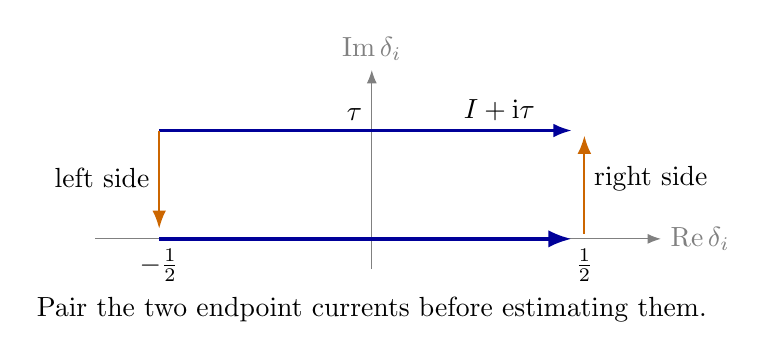
\begin{tikzpicture}[x=5.4cm,y=3.2cm,>=Latex]
 \draw[->,gray] (-.65,0)--(.68,0) node[right] {$\Rea\delta_i$};
 \draw[->,gray] (0,-.12)--(0,.67) node[above] {$\Ima\delta_i$};
 \draw[very thick,blue!60!black,->] (-.5,0)--(.47,0);
 \draw[thick,blue!60!black,->] (-.5,.43)--(.47,.43);
 \draw[thick,orange!80!black,->] (-.5,.43)--(-.5,.04);
 \draw[thick,orange!80!black,->] (.5,.02)--(.5,.41);
 \node[below] at (-.5,0) {$-\tfrac12$};
 \node[below] at (.5,0) {$\tfrac12$};
 \node[above] at (.3,.43) {$I+\ii\tau$};
 \node[left] at (-.5,.24) {left side};
 \node[right] at (.5,.24) {right side};
 \node[above left] at (0,.43) {$\tau$};
 \node[align=center] at (0,-.28)
 {Pair the two endpoint currents before estimating them.};
\end{tikzpicture}

\caption{One coordinate is moved on its whole original interval.
Both horizontal arrows give the direction of their integrals.
The vertical arrows give the boundary contribution that is subtracted.
The two vertical sides are retained and paired by
\eqref{of:paired-current}. Spectator variables remain on their
whole real intervals. Only after the distant charges have been
summed is a small real cube introduced.}
\end{figure}

Apply Lemma~\ref{of:endpoints} in every spectator coordinate.
Using
\[
 |\sinh(2\pi v)\sinh(\pi n_iNv)|
             \le C_{\boldsymbol n}|n_i|Nv^2 e^{\pi|n_i|Nv},
\]
the absolute value of the weighted paired-side contribution is at most
\begin{equation}\label{of:vertical-bound}
 C_{\boldsymbol n}|n_i|N\ell_i\,e^{N(\Phi-\gamma_e)}
       \prod_{j\ne i}|\ell_j|^{-2}
       \int_0^\tau v^2e^{-2\pi N(\ell_i-|n_i|/2)v}\,dv.
\end{equation}
For $\ell_i>|n_i|/2+D$, $D\ge1$, the integral is at most
$2/[2\pi N(\ell_i-|n_i|/2)]^3$. The resulting charge sum is finite:
\begin{equation}\label{of:tail-series}
 \sum_{\ell>|n_i|/2+D}\frac{\ell}{(\ell-|n_i|/2)^3}
                \le C\left(D^{-1}+(|n_i|+1)D^{-2}\right).
\end{equation}
For example, write $\ell=(\ell-|n_i|/2)+|n_i|/2$ and compare
the sums of the inverse squares and cubes with their decreasing
integrals. A change in the integer endpoint only changes the absolute
constant. The spectator sums converge by their inverse-square factors.

On the upper horizontal interval use \eqref{of:entire-bound}, with
fixed Cauchy neighborhoods for spectator source derivatives. They can
be chosen to give total exponential cost at most $2\pi r\tau N$.
The shifted Gaussian and Fourier factors in the distinguished
coordinate have modulus at most
$e^{\pi|n_i|N\tau-2\pi\ell_iN\tau}$. Thus its weighted contribution
is at most
\begin{equation}\label{of:horizontal-bound}
 C_{\boldsymbol n}\ell_i\prod_{j\ne i}|\ell_j|^{-2}
 \exp\left(N\left[\Phi+b_N+2\pi r\tau
               -2\pi\tau(\ell_i-|n_i|/2)\right]\right).
\end{equation}
Choose the fixed number $D$ so large that
$2\pi\tau D>2\pi r\tau+2\gamma_e$, and put
$M_i=\lceil|n_i|/2+D\rceil$. Summing the geometric tail in
\eqref{of:horizontal-bound} gives a strict exponential gap.
Equations \eqref{of:vertical-bound}--\eqref{of:tail-series} give
the same for both vertical sides together.

Negative distant charges satisfy the identical estimates, by reflection.
Taking a union bound over the distinguished coordinate proves
\begin{proposition}[The entire distant-charge tail]\label{of:far}
For some fixed $\gamma_\infty>0$ and each fixed sufficiently long
twist tuple, the sum of the absolute values of all complete weighted
charge terms for which $|\ell_i|>M_i$ for at least one $i$ is at most
\[
            C_{\boldsymbol n}N^C e^{N(\Phi-\gamma_\infty)}.
\]
Every spectator charge is summed over its full nonzero integer range.
\end{proposition}

The union bound can count a charge more than once; this only enlarges
an upper bound. No infinite sum on a sharply truncated small cube has
been formed. The absolute convergence already proved and the displayed
summable majorants justify each sum and interchange.

\section{The remaining charges outside the local range}

After Proposition~\ref{of:far}, only
$0<|\ell_i|\le M_i$ remain. This is a finite set because the twist
tuple was fixed before $N$ varies. Choose a new inner radius $b$ with
$0<b<a/4$, independently of the outer radius $B$, and let
$K_b=[-b,b]^r$.

Suppose one remaining charge satisfies $|\ell_i|/|n_i|>a$.
Reflection permits us to take $\ell_i>0$ for the absolute estimate.
On the real domain outside $K_b$, \eqref{of:gap} gives a fixed loss.
Inside $K_b$, shift only the $i$th coordinate by $\ii b/|n_i|$.
For $|x_j|\le b$ and $0\le v\le b/|n_i|$,
\eqref{of:complex-taylor-bound} gives
\[
 \Rea A_N(x+\ii ve_i)\le A_N(0)-c|x|^2+Cv^2.
\]
The real chirp and charge contribution is
\begin{equation}\label{of:bad-charge-loss}
 -2\pi n_ix_iv-2\pi\ell_iv
                  \le-2\pi|n_i|(a-b)v\le0.
\end{equation}
On the translated horizontal face, the loss is at least
$2\pi b(a-b)$ and the source cost is at most $Cb^2/n_0^2$.
On a vertical side $|x_i|=b$, the fixed loss $cb^2$ persists,
while \eqref{of:bad-charge-loss} remains nonpositive. Increase
$n_0$ so that these costs are smaller than half the indicated losses.
The amplitudes in \eqref{of:packet} cost only a power of $N$.
Both side faces and the translated interval are therefore bounded
by a rate $\Phi-\gamma_{\rm bad}$ with $\gamma_{\rm bad}>0$ fixed.

There are finitely many such bounded charges, so their whole sum has
the same strict exponential upper rate, with a constant depending on
$\boldsymbol n$. Using the inner cube here and the outer cube for
the local saddle avoids a conflict between the two contour estimates.

\section{The unit charges and proof of the theorem}

All remaining charges lie in the local range
$|\ell_i|/|n_i|\le a$. They are still a finite set for fixed
$\boldsymbol n$. Apply Lemma~\ref{of:local-integral} inside $K_B$
and \eqref{of:gap} to its real exterior. Every charge with a
magnitude greater than one has, by Lemma~\ref{of:charge-gap}, a
positive fixed-tuple gap below the all-unit critical value. The
smallest such gap may tend to zero when a twist magnitude tends to
infinity; it remains positive in the limit under consideration,
where the tuple is fixed.

The $2^r$ choices of unit signs contribute exactly equally. Indeed,
in one coordinate replace $\ell_j$ by $-\ell_j$ and substitute
$\delta_j\mapsto-\delta_j$ on its full symmetric interval.
The source and the Gaussian are even, the sine changes sign, and
the charge factor changes sign. Those two signs cancel.
The parity character is unchanged because the two exponents differ
by $2(N+1)\ell_j$. This is an equality of the original integrals,
including phase, before any approximation.

For the positive unit vector, the original parity is
$(-1)^{(N+1)r}$. Multiplying its local formula by $2^r$, the
prefactor $\Gamma_N(-\ii)^r$, and that parity gives
\eqref{of:asymptotic}. Choose $n_0$ large enough that the unit
loss $O(\sum_j n_j^{-2})$ is smaller than one quarter of every
fixed gap used for the far charges, the bounded nonlocal charges,
the side faces and the exterior of $K_B$. Also require $a n_0\ge1$.
The first charge then lies in the local range and dominates all these
parts for sufficiently large $N$. The other finitely many local
charges are controlled by their own strictly positive gaps.
Polynomial factors can be absorbed by reducing a positive exponential
gap. This proves the error statement in Theorem~\ref{of:main}.

The limiting coefficient is nonzero by
Lemma~\ref{of:local-integral}, and every factor outside the action
has zero exponential rate. Taking absolute values, logarithms and
dividing by $N$ proves \eqref{of:rate}. The estimate for the unit
action drop follows from Lemma~\ref{of:charge-gap} after passage
to the limit. This completes the proof.

\section{Use for a marked knot source}

We record the exact interface with the motivating source so that
the theorem can be cited without importing a geometric conclusion
into an analytic premise. Suppose a marked diagram has $r$ crossing
regions and an exact full polynomial source $S_N$. The marked coefficient
and its reduced framing convention are supplied by
\cite[Theorems 9.1 and 10.1, Corollary 9.2]{FinitePaper}.
Choose the central degree
region in every local factor and let $P_N$ be its shared coefficient.
This is a linear part of the original source; it need not define an
independent invariant under changes of diagram.

In that application the required local expansion has the form
\begin{equation}\label{of:face-packet}
 C_N(\delta)=
 \frac{(-1)^{(N-1)r}N^{2r}e^{NA_N(\delta)}}
 {(2\pi N)^{(r-1)/2}\sqrt{\det H_N(\delta)}}
                          (1+O(N^{-1})).
\end{equation}
The matrix $H_N$ is the normalized face Hessian on the quotient by
common scale. A separate source theorem must construct that quotient,
prove its nondegeneracy, choose the positive complete branch of the
determinant root, and establish this expansion on a fixed complex
neighborhood. It must also prove the global shared gap
\eqref{of:gap}. Nodal values or a formal stationary phase alone
would not establish either premise.

If these inputs hold, set
\[
 \alpha=(3r+1)/2,\qquad \varepsilon_N=(-1)^{(N-1)r},\qquad
 a_N=(2\pi)^{-(r-1)/2}(\det H_N)^{-1/2}.
\]
The two level-parity factors in \eqref{of:asymptotic} multiply to
one. The complete central filling contribution is therefore
\begin{equation}\label{of:source-result}
\begin{split}
 \mathcal I_N^{\rm central}
 ={}&\Gamma_N(-2\ii)^r\sqrt{2\pi}N^{r+1/2}
   \frac{\prod_j\sin(2\pi z_{N,j})}
        {\sqrt{\det H_N(z_N)}\sqrt{\det Q_N}}e^{NS_N}\\
 &\qquad\times
       (1+O_{\boldsymbol n}(N^{-1})
                       +O_{\boldsymbol n}(e^{-\kappa_{\boldsymbol n}N})).
\end{split}
\end{equation}
This derivation includes even and odd levels and their original
double-root derivatives. The single reduced mark and the face-lattice
normalization belong to the exact finite source theorem and are not
inserted again in \eqref{of:source-result}.

Two further statements are required for a full knot volume theorem.
First, the classical critical equations must construct the smooth
filling of the same marked crossing circles and establish
\[
                  2\pi\Rea S_0=\operatorname{Vol}(S^3\setminus K).
\]
Second, the entire difference between the full source and its central
part must be bounded after filling. If that remainder has a strictly
smaller upper rate, the triangle and reverse triangle inequalities
give the full invariant's limit; see
\cite[Proposition 11.2]{FinitePaper}. The unit framing character
does not change the logarithmic absolute rate. Neither the geometric
identity nor that complementary-source estimate is a conclusion of
Theorem~\ref{of:main}.

\begin{thebibliography}{9}
\bibitem{FinitePaper}
\emph{Finite spectral evaluation and uniform filling bounds}, companion
manuscript, 2026.
\href{https://sashakolpakov.github.io/murakamis_dream/papers/filling-bounds.pdf}{Full text}.
\bibitem{DLMF}
F.~W.~J. Olver et al., eds., \emph{NIST Digital Library of Mathematical
Functions}, Chapter 2, Asymptotic Approximations, \S2.4, Contour Integrals.
\href{https://dlmf.nist.gov/2.4}{dlmf.nist.gov/2.4}.
\bibitem{Hormander}
L. H\"ormander, \emph{The Analysis of Linear Partial Differential
Operators I: Distribution Theory and Fourier Analysis}, Springer,
2003 reprint of the second edition.
\href{https://doi.org/10.1007/978-3-642-61497-2}{doi:10.1007/978-3-642-61497-2}.
\end{thebibliography}
\end{document}
